\documentclass[10pt]{beamer}

% Copia local de preamble.tex:
\usetheme[progressbar=frametitle]{metropolis}
\usepackage{appendixnumberbeamer}
\usepackage{fancyvrb}
\usepackage{booktabs}
\usepackage[scale=2]{ccicons}
\usepackage{pgfplots}
\usepgfplotslibrary{dateplot}
\usepackage{type1cm}
\usepackage{lettrine}
\usepackage{ragged2e}
\usepackage{xspace}
\newcommand{\themename}{\textbf{\textsc{metropolis}}\xspace}
\usepackage{graphicx} % Allows including images
\usepackage{booktabs} % Allows the use of \toprule, \midrule and \bottomrule in tables
\usepackage[utf8]{inputenc} %solucion del problema de los acentos.
\usepackage{xcolor}
\definecolor{LightGray}{gray}{0.9}

\usepackage{minted}
\usemintedstyle{tango}
\newcommand{\mypyfile}[1]{\inputminted[linenos=true, fontsize=\footnotesize, frame=lines, framesep=5\fboxrule,framerule=1pt]{python}{#1}}

\setminted[python]{breaklines,frame=lines,framesep=2mm,baselinestretch=1.2,bgcolor=LightGray,linenos, fontsize=\footnotesize} % obeytabs=true, tabsize=2, showtabs=true}

%%%%%%%%%%%%%%%%%%%%%%%%%%%%%%%%%%%%%%%%%%%%%%%%%%%%%%%%%%%%%%%%%%%%%%%%%%%%%%%%%%%%%%
\setbeamercolor{progress bar}{fg=blue!50!black,bg=white!50!black}
\setbeamercolor{title separator}{fg=red!50!black,bg=white!50!black}
\setbeamercolor{frametitle}{fg=white!80!black,bg=red!50!black}
\title[PCFI161]{Programaci\'on para F\'isica y Astronom\'ia}
\subtitle{Departamento de Física.}

\newcommand{\myfront}{
\author[PCFI161]{Corodinadora: C Loyola \\ Profesoras/es C Loyola / C Femenías / Y Navarrete / C Ruiz}
\institute[UNAB]{Universidad Andrés Bello}
\date{Primer Semestre 2025}
}

\titlegraphic{%
  
\includegraphics[width=.08\textwidth]{logo-tux.png}\hfill
  
\includegraphics[width=.3\textwidth]{logo-unab.png}\hfill
  
\includegraphics[width=.08\textwidth]{logo-python.png}
}

\makeatletter
\setbeamertemplate{title page}{
  \begin{minipage}[b][\paperheight]{\textwidth}
    \vfill%
    \ifx\inserttitle\@empty\else\usebeamertemplate*{title}\fi
    \ifx\insertsubtitle\@empty\else\usebeamertemplate*{subtitle}\fi
    \usebeamertemplate*{title separator}
    \ifx\beamer@shortauthor\@empty\else\usebeamertemplate*{author}\fi
    \ifx\insertdate\@empty\else\usebeamertemplate*{date}\fi
    \ifx\insertinstitute\@empty\else\usebeamertemplate*{institute}\fi
    \vfill
    \ifx\inserttitlegraphic\@empty\else\inserttitlegraphic\fi
    \vspace*{1cm}
  \end{minipage}
}
\makeatother


\makeatletter
\setlength{\metropolis@titleseparator@linewidth}{2pt}
\setlength{\metropolis@progressonsectionpage@linewidth}{2pt}
\setlength{\metropolis@progressinheadfoot@linewidth}{2pt}
\makeatother


\begin{document}

\myfront{}

\begin{frame}
  \titlepage
\end{frame}

\begin{frame}
  \frametitle{Resumen - Parte 2}
  \tableofcontents
\end{frame}

%----------------------------------------------------------------------------------------
%	PRESENTATION SLIDES
%----------------------------------------------------------------------------------------

\metroset{block=fill}

%------------------------------------------------
\section{El ambiente GNU/Linux, editores y manejo de archivos.} 

\subsection{GNU/Linux} 

\begin{frame}{El ambiente GNU/Linux}
\begin{itemize}
	\item GNU es un sistema completo de software libre compatible con Unix (Stallman, 1983).
	\item Linus Torvalds programó Linux (1991), un kernel Unix-like. Con GNU completó el sistema.
	\item Hoy existen múltiples distribuciones: Debian, Ubuntu, Fedora, etc.
\end{itemize}
\end{frame}

\begin{frame}{El ambiente GNU/Linux}
\begin{itemize}
	\item Ofrece interfaz de línea de comandos (CLI) y gráfica (GUI).
	\item La CLI más usada es \textbf{bash} (Bourne Again Shell).
	\item Para usar la shell en entorno gráfico se necesita un emulador de terminal, p.e. \texttt{gnome-terminal}.
\end{itemize}
\end{frame}

\begin{frame}[fragile]{A tener en cuenta en GNU/Linux}
\begin{itemize}
	\item En Linux todo es un fichero: directorios, dispositivos, etc.
	\item Estructura jerárquica en forma de árbol: \texttt{/} (raíz).
	\begin{example}[Linux]
	\texttt{/home/usuario/archivo.dat}
	\end{example}
	\begin{example}[Windows]
	\texttt{C:\textbackslash Users\textbackslash usuario\textbackslash archivo.dat}
	\end{example}
\end{itemize}
\end{frame}

\begin{frame}{A tener en cuenta en GNU/Linux}
\begin{itemize}
	\item Existe un súperusuario llamado \texttt{root}.
	\item El usuario \texttt{root} puede instalar/eliminar programas, crear usuarios, etc.
	\item Muchas distribuciones usan \texttt{sudo} para que un usuario pueda ejecutar órdenes como \texttt{root}.
\end{itemize}
\end{frame}

\subsection{Utilidades GNU/Linux}

\begin{frame}[fragile]{Utilidades GNU/Linux}
\begin{itemize}
	\item \texttt{sudo} ejecuta un comando con privilegios de \texttt{root}.
	\item \texttt{apt-get} instala paquetes desde repositorios, sin descargar manualmente.
\end{itemize}
\begin{alertblock}{Modo de uso \texttt{apt-get}}
\texttt{apt-get [options] command}
\end{alertblock}
\begin{example}
\texttt{sudo apt-get install vim}
\end{example}
\end{frame}

\subsection{La shell de linux}
\begin{frame}{La \textit{shell} de linux}
\metroset{block=fill}
\begin{block}{Comandos básicos}
  \begin{table}
	\resizebox{\linewidth}{!}{
	  \begin{tabular}{ll}
		\toprule
		\textbf{Comando} & \textbf{Descripción} \\ \midrule
		\texttt{ls}      & Listar directorios (opciones: -a, -R, -t, -r) \\
		\texttt{pwd}     & Imprime el directorio de trabajo actual       \\
		\texttt{cd}      & Cambia/Ingresa a un directorio                \\
		\texttt{mv}      & Mueve o renombra un archivo/directorio        \\
		\texttt{cp}      & Copia un archivo o carpeta                    \\
		\texttt{rm}      & Elimina archivos o directorios                \\
		\texttt{mkdir}   & Crea un directorio                            \\
		\texttt{rmdir}   & Elimina un directorio vacío                   \\
		\bottomrule
	  \end{tabular}
	}
  \end{table}
\end{block}
\end{frame}

\begin{frame}[fragile]{La \textit{shell} de linux}
\begin{example}[comando man]
\begin{verbatim}
>$ man ls
>$ man cd
>$ man pwd
\end{verbatim}
\end{example}
\end{frame}

\subsection{Editores de texto}
\begin{frame}{Editores de texto}
\begin{itemize}
	\item Hay muchos: nano, pico, vim, emacs, etc.
	\item Vim (Vi IMproved) es un editor muy popular en terminal.
	\item Separa modos de edición y comandos. Ideal para programación en entornos remotos.
\end{itemize}
\end{frame}

\begin{frame}{VIM}
\begin{itemize}
	\item VIM = Vi IMproved
	\item Permite editar, compilar y corregir rápidamente.
	\item Existen tutoriales como \texttt{vimtutor}, sitios como \texttt{openvim.com}, etc.
\end{itemize}
\end{frame}

\section{Instalando GNU/Linux}
\subsection{Usando VMWARE Workstation Player}

\begin{frame}[fragile]{VMWARE}
	\begin{block}{M\'aquinas virtuales}
		Permiten correr un SO dentro de otro (p.ej. GNU/Linux dentro de Windows).
	\end{block}
\end{frame}

\begin{frame}[fragile]{Instalando VMWARE}
	\begin{itemize}
		\item Descargue VMWARE Workstation Player.
		\item Descargue la ISO de Ubuntu (u otra distro).
		\item Instale la m\'aquina virtual.
	\end{itemize}
\begin{block}{Video sugerido}
\url{https://www.youtube.com/watch?v=2ykto1mD4pc}
\end{block}
\end{frame}

\begin{frame}[fragile]{Ubuntu Inside Windows10}
\begin{itemize}
	\item Usar WSL con Windows 10 y un entorno gráfico como GWSL.
	\item Muy útil para desarrollo en Linux dentro de Windows.
\end{itemize}
\end{frame}

\begin{frame}{Ubuntu Inside Windows10}
\begin{figure}
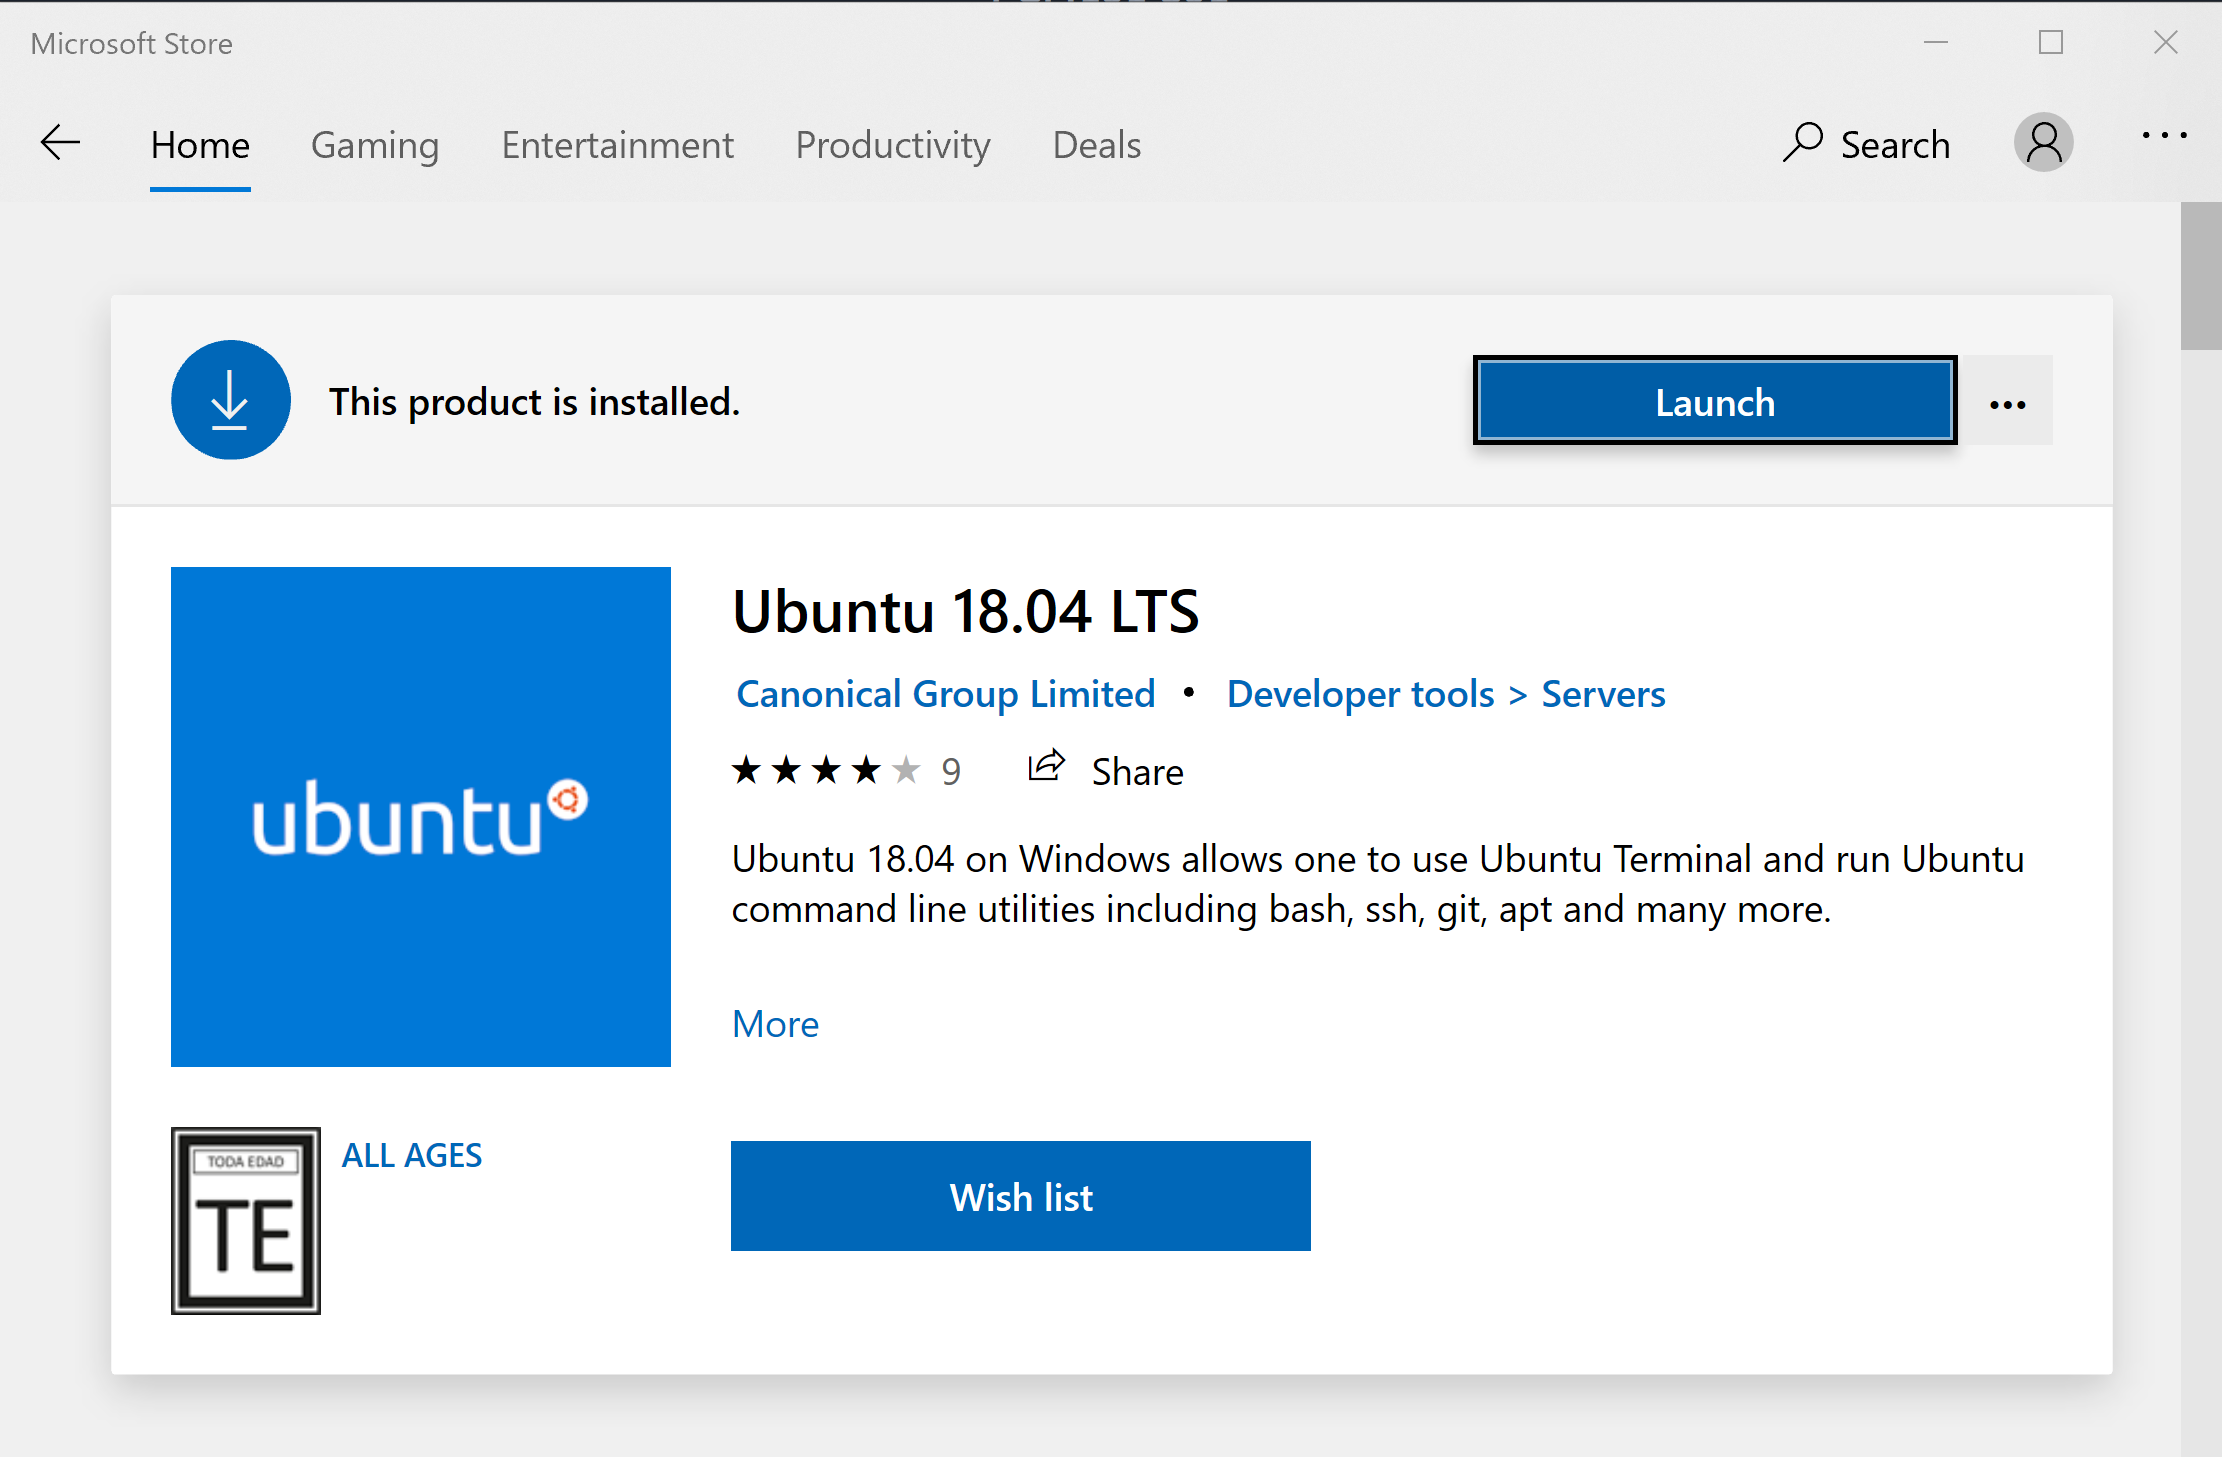
\includegraphics[width=0.9\textwidth]{ubuwin01.png}
\end{figure}
\end{frame}

\begin{frame}[fragile]{Ubuntu Inside Windows11}
\begin{block}{Instalando WSL}
\texttt{wsl --install}
\end{block}
\end{frame}

\begin{frame}
\begin{figure}
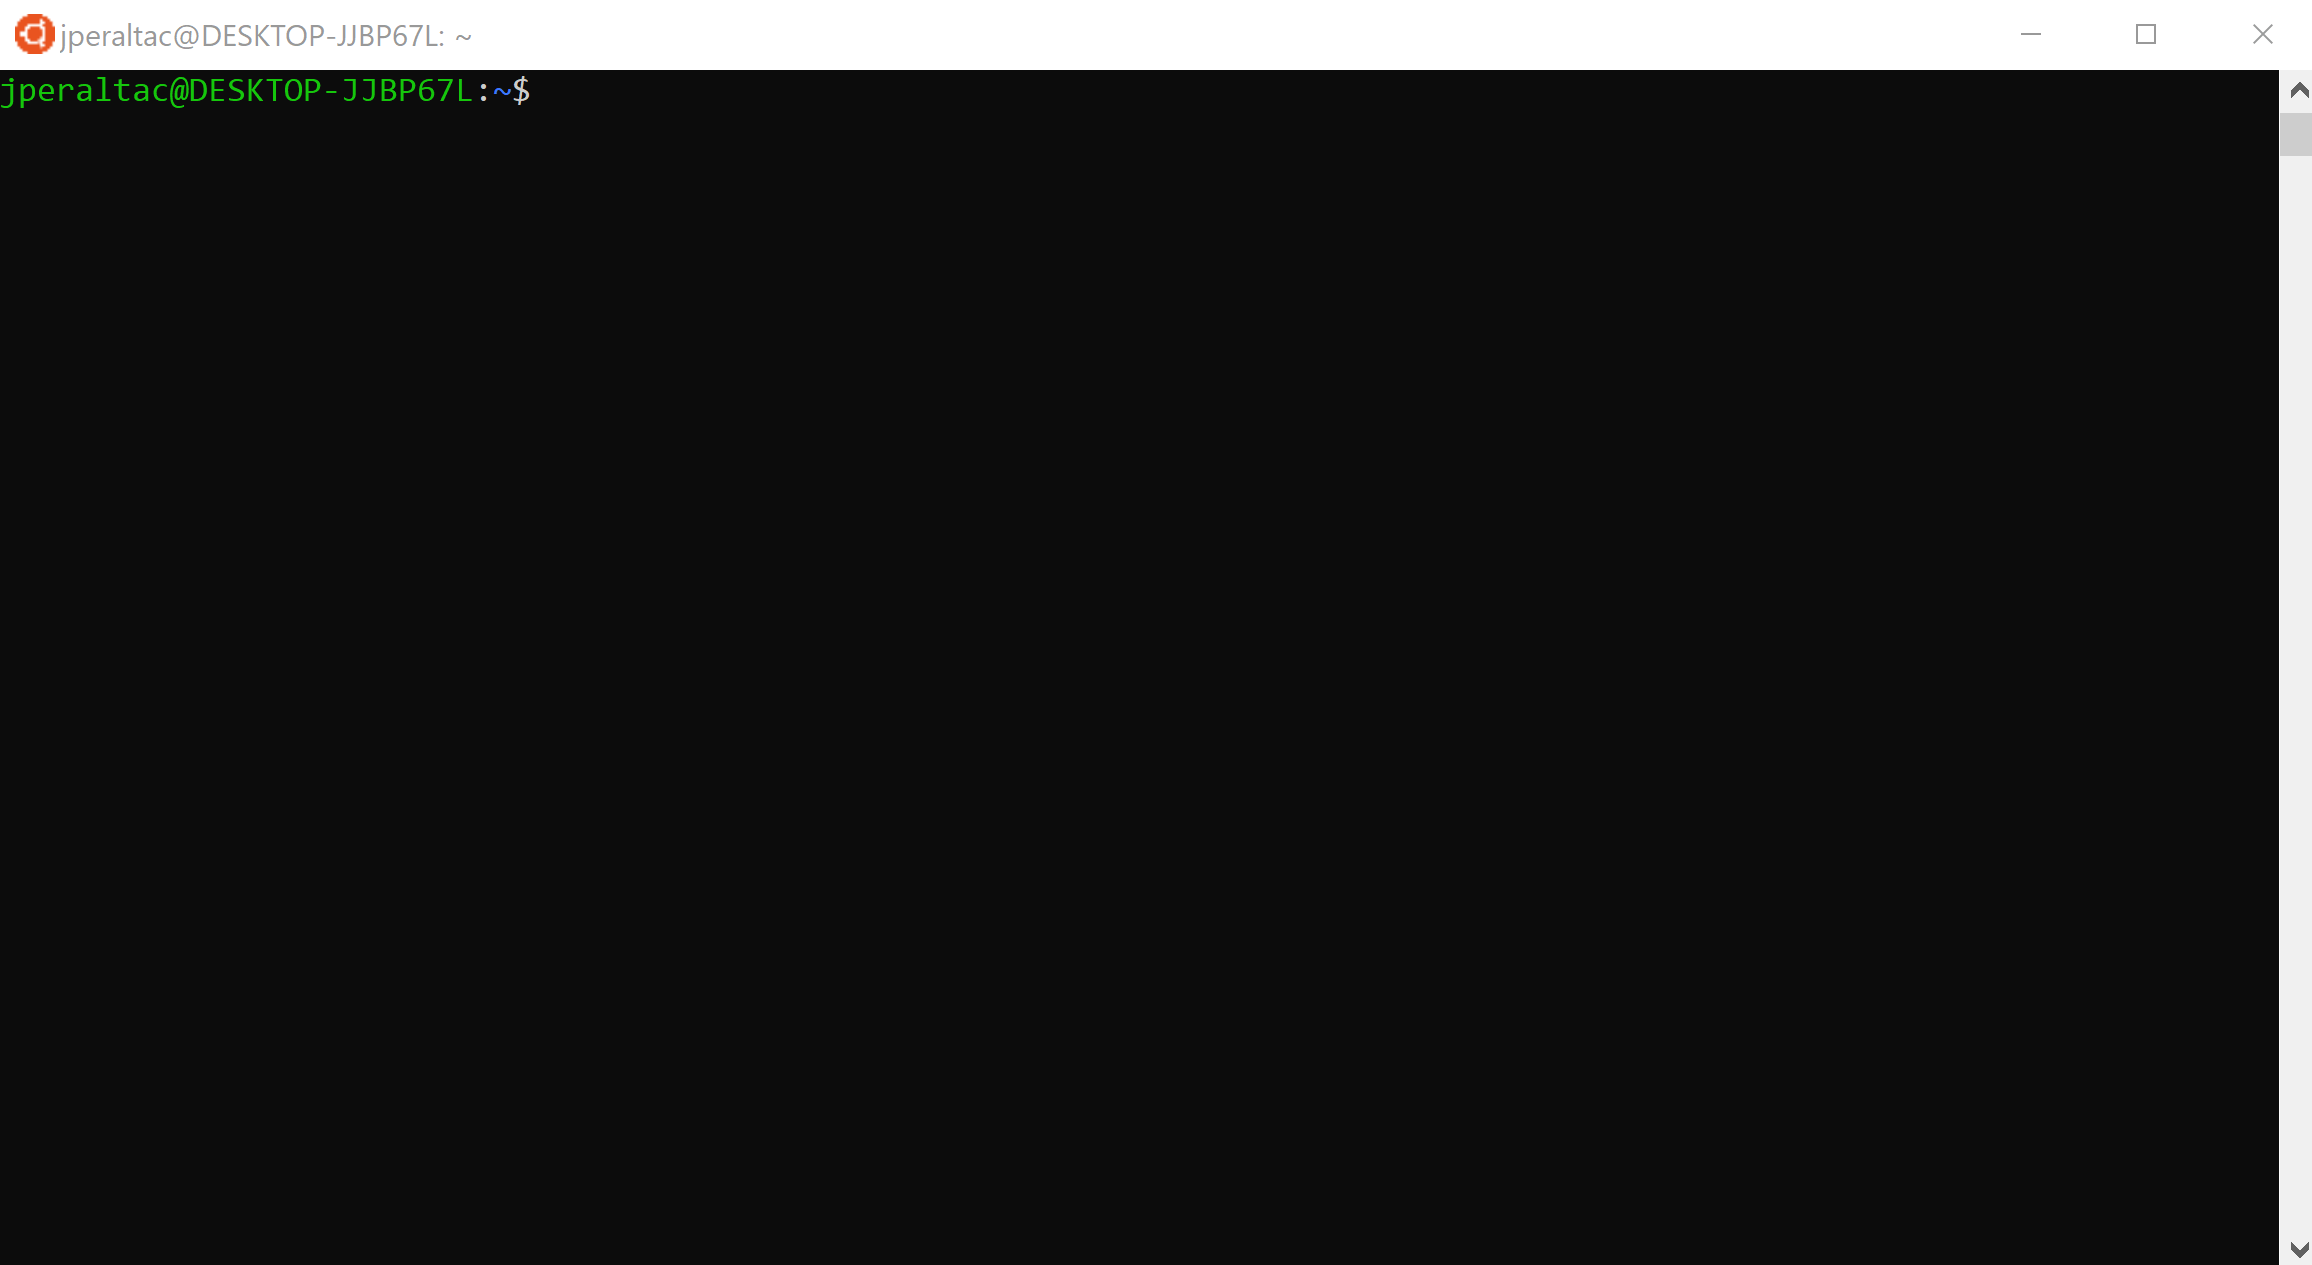
\includegraphics[width=0.9\textwidth]{ubuwin02.png}
\end{figure}
\end{frame}

\section{Google Colab}

\begin{frame}[fragile]
\frametitle{Google Colab}
\begin{itemize}
    \item Servicio de Google para programar en Python en la nube (via Jupyter).
    \item Permite usar GPU gratis para proyectos de IA, etc.
\end{itemize}
\end{frame}

\begin{frame}[fragile]
\frametitle{Google Colab}
\begin{figure}
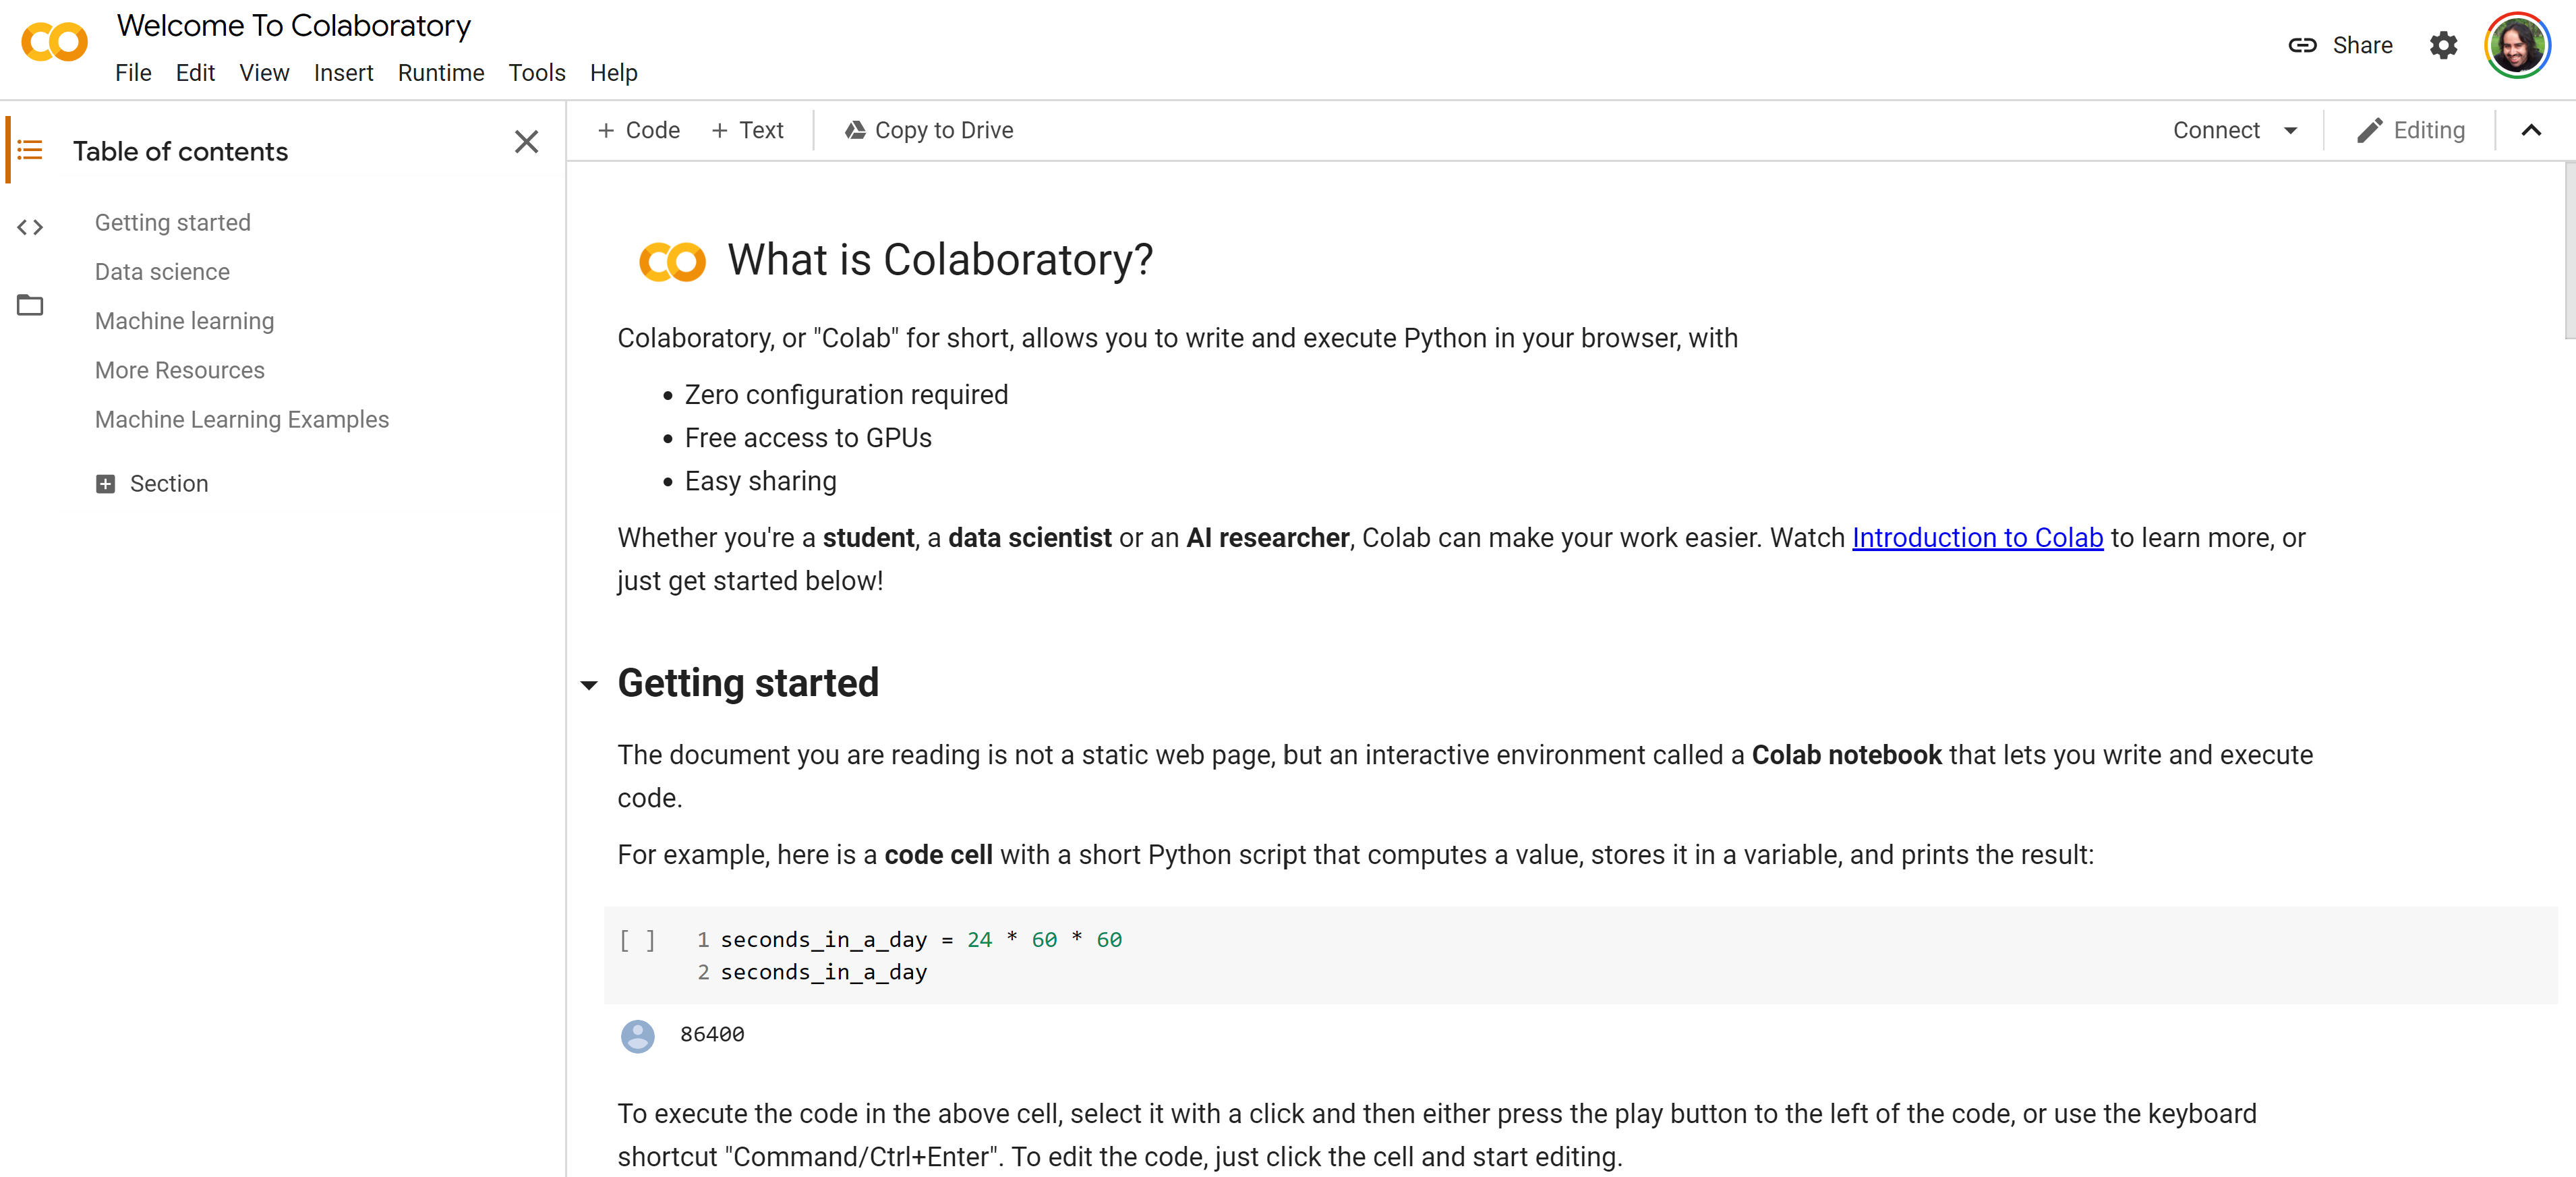
\includegraphics[width=1\textwidth]{GColab01.png}
\end{figure}
\end{frame}

\begin{frame}[fragile]
\frametitle{Google Colab}
\begin{figure}
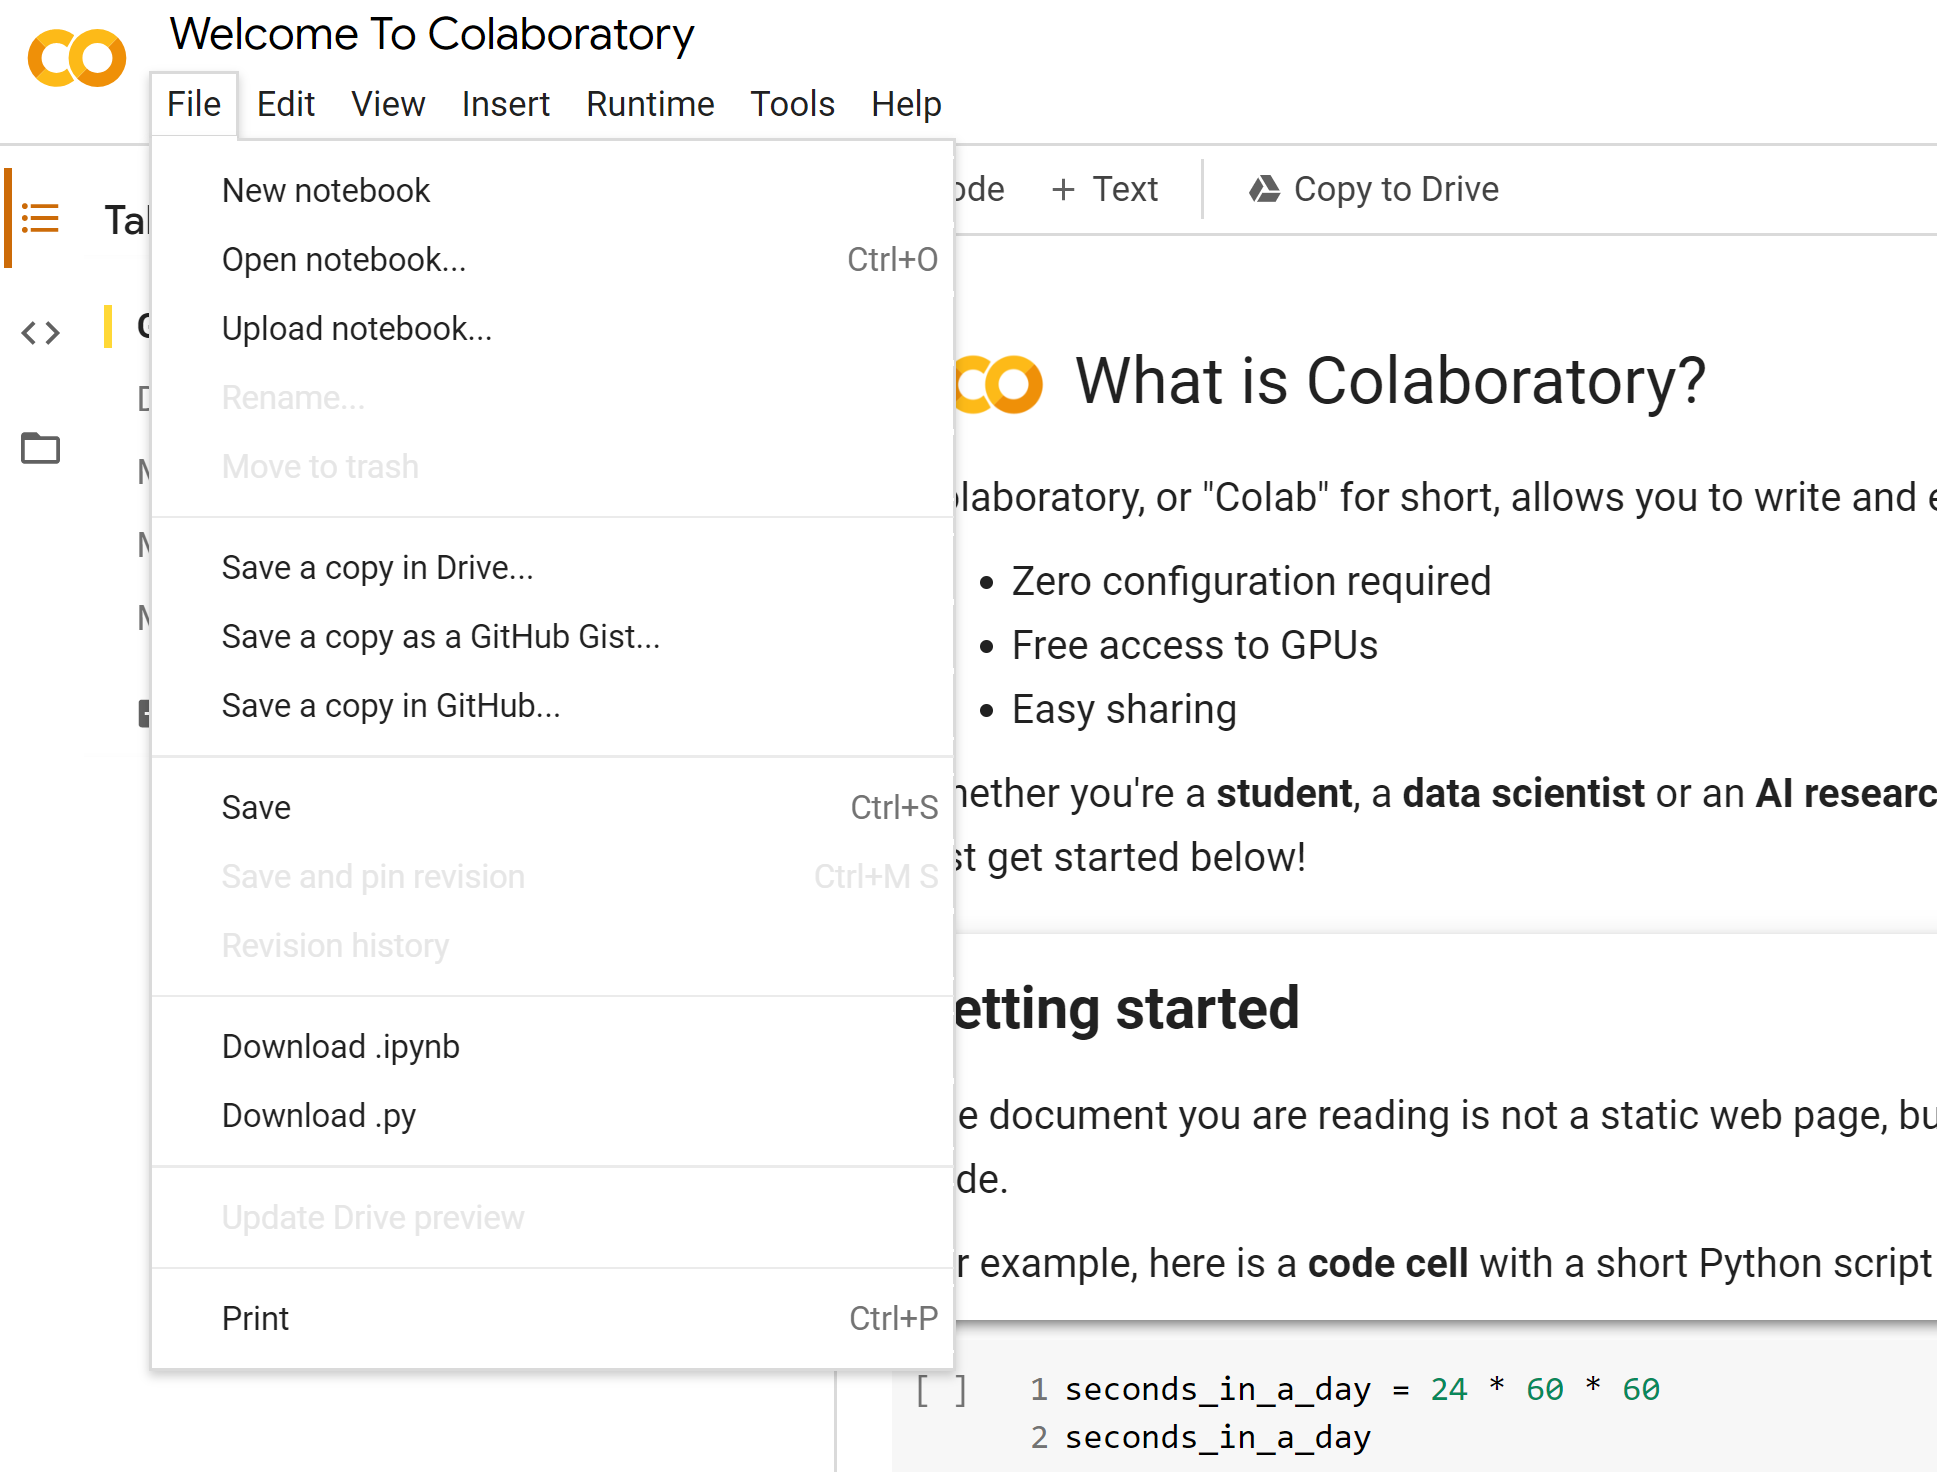
\includegraphics[width=1\textwidth]{GColab02.png}
\end{figure}
\end{frame}

\begin{frame}[fragile]
\frametitle{Google Colab}
\begin{figure}
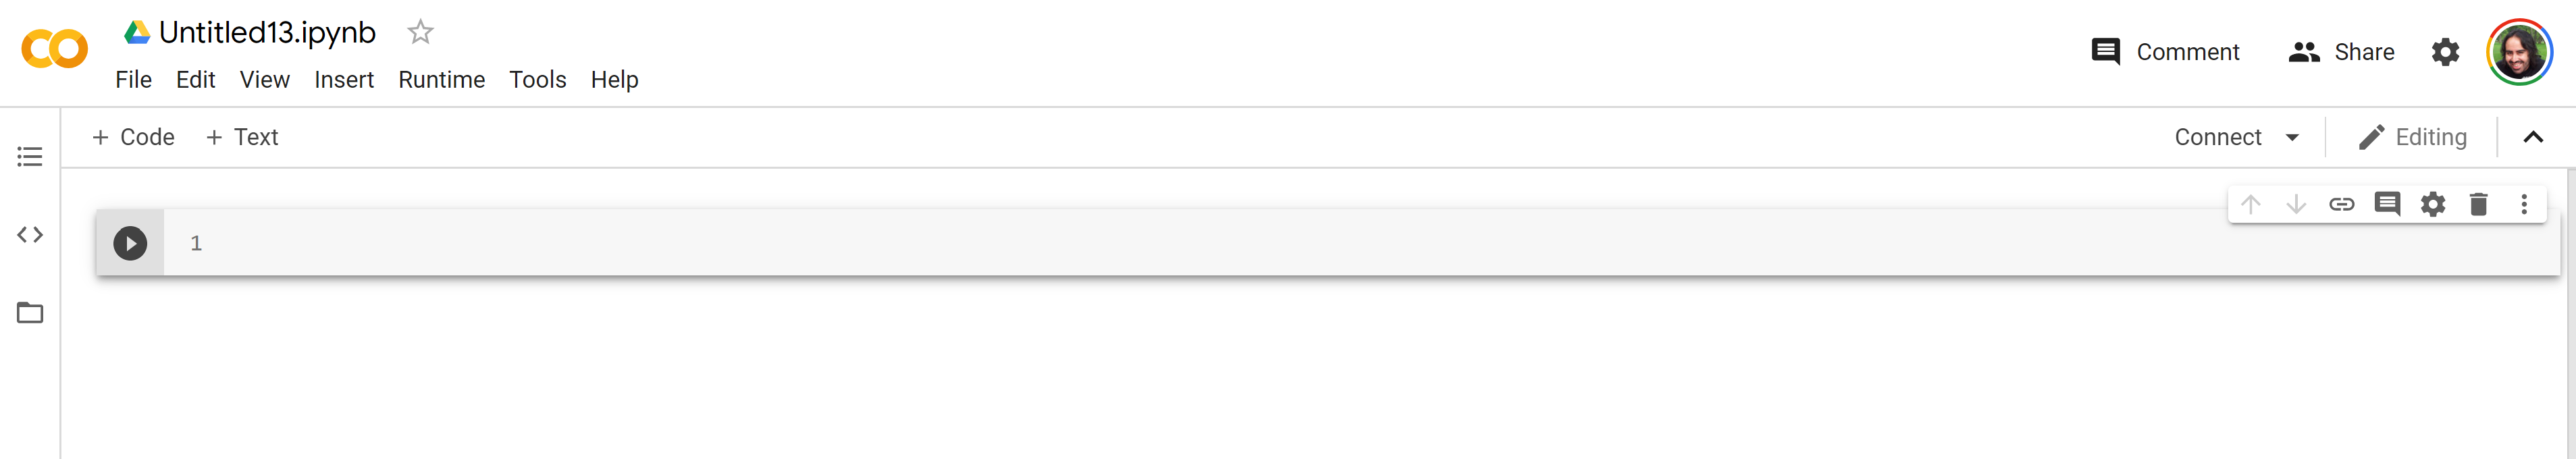
\includegraphics[width=1\textwidth]{GColab03.png}
\end{figure}
\end{frame}

\begin{frame}[fragile]
\frametitle{Google Colab}
\begin{figure}
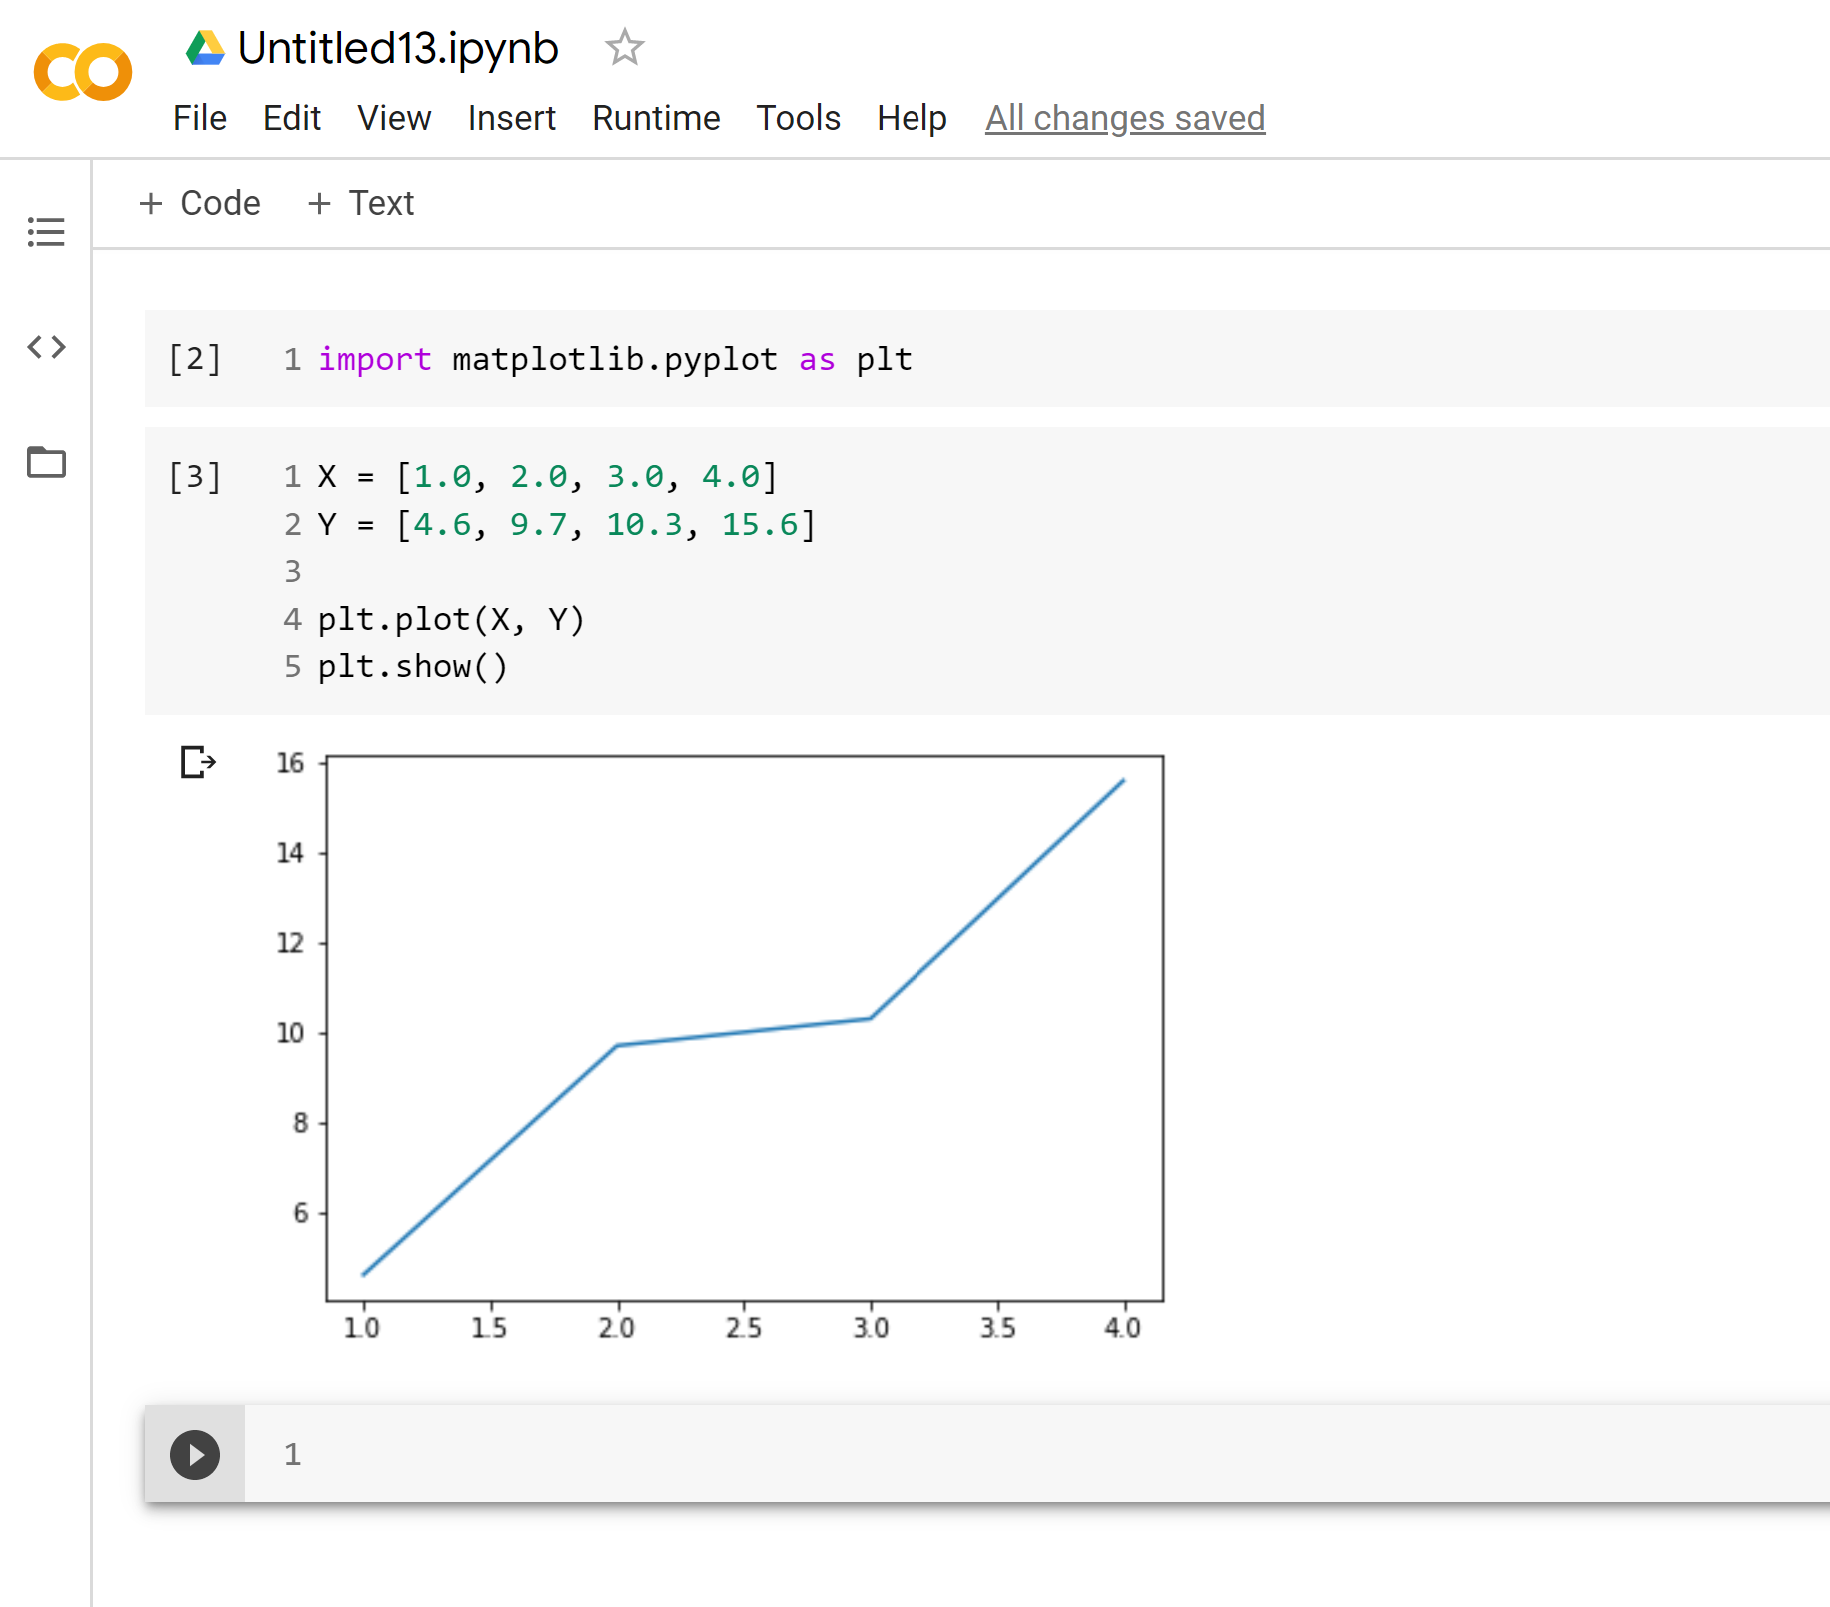
\includegraphics[width=0.7\textwidth]{GColab04.png}
\end{figure}
\end{frame}

\begin{frame}
\frametitle{Manos a la obra}
\begin{itemize}\small
    \item Instalar alguna forma de GNU/Linux (WSL, VM, dual boot).
    \item Crear directorios y archivos, moverte en la línea de comandos, renombrar, etc.
\end{itemize}
\end{frame}

\begin{frame}
\frametitle{Actividades de refuerzo}
\begin{itemize}\small
    \item \textbf{Actividad 1:} Crear un directorio \texttt{MiProyecto}, allí un subdirectorio \texttt{src}, y un archivo de texto \texttt{README.md}.
    \item \textbf{Actividad 2:} Abre \texttt{README.md} con \texttt{vim} o \texttt{nano}, escribe tu nombre y guarda.
    \item \textbf{Actividad 3:} Usa \texttt{man} para investigar más sobre \texttt{ls}, \texttt{cp}, \texttt{mv}.
\end{itemize}
\end{frame}

\begin{frame}
\Huge{\centerline{Fin de la Parte 2}}
\end{frame}

\end{document}

